\documentclass[12pt, compress]{beamer}

\usetheme{Warsaw}
\usepackage{amsmath, amssymb, amsfonts}
\usepackage[spanish, english]{babel}
\usepackage{color}
\usepackage{graphicx}
\usepackage[utf8]{inputenc}
\usepackage{mathtools}
\usepackage{multirow}
\usepackage[round, comma]{natbib}
\usepackage{tabularx}
\usepackage{tabulary, comment, algpseudocode, algorithm, bm}
\usepackage{bbm}

\usepackage{tikz}
\usepackage{threeparttable}
\usepackage{caption}
\usetikzlibrary{positioning, arrows.meta}
\usepackage{tikz}
\usetikzlibrary{shapes.geometric, arrows.meta}
\usepackage{pgfplots}
\pgfplotsset{compat=1.18} % or another version you have
\usetikzlibrary{arrows.meta}

\usepackage{etoolbox}

% Patch to allow non-floating algorithmic in beamer
\makeatletter
\patchcmd{\ALG@beginalgorithmic}{\begin{trivlist}}{\begin{minipage}{\linewidth}\tiny}{}{}
		\patchcmd{\ALG@endalgorithmic}{\end{trivlist}}{\end{minipage}}{}{}
\makeatother

% Reduce size of line numbers
\algrenewcommand\alglinenumber[1]{\scriptsize #1}

% Avoid floating in Beamer
\makeatletter
\setbeamertemplate{caption}[numbered]
\newcommand{\nonfloatalgorithm}[1]{%
	\par\vspace{\baselineskip}
	\noindent\begin{minipage}{\linewidth}
		\begin{algorithmic}[1] #1 \end{algorithmic}
	\end{minipage}\par\vspace{\baselineskip}
}
\makeatother

\let\Tiny \tiny
%\setbeamertemplate{background canvas}{\includegraphics[width = \paperwidth, height = \paperheight]{EAFIT.pdf}} % Include an image as part of the background
\setbeamertemplate{navigation symbols}{} % Getting rid of navigation symbols
\useoutertheme{tree}
\setbeamertemplate{footline}[frame number]

%%%%%%%%%%%%%%%%%%%%%%%% PRESENTACION %%%%%%%%%%%%%%%%%%%%%%%%%%%%
\title{Causal inference}
\subtitle{Kaunas University of Technology}
\date{2026}
\author[Andr\'e Ram\'irez H.]{\textbf{Andr\'es Ram\'irez-Hassan}}
\institute[EAFIT]{\small{Universidad EAFIT\\School of Finance, Economics and Government}}
%%%%%%%%%%%%%%%%%%%%%%% DOCUMENTO %%%%%%%%%%%%%%%%%%%%%%%%%%%%%%%%%

%\decimalpoint
%\justifying
\begin{document}
	
	%\tikzstyle{every picture}+=[remember picture]
	%\everymath{\displaystyle}
	%\tikzstyle{na} = [baseline=-.5ex]
	\maketitle
	
	% \begin{frame}
		% \includegraphics[width= 0.15\linewidth]{escudo.eps}
		% \maketitle
		% \end{frame}
	
	
	
	\section*{Outline}
	\begin{frame}
		\textbf{\Large{Outline}}
		\tableofcontents
	\end{frame}
	
\section{Introduction}
	
\begin{frame}
	\frametitle{Introduction}

\begin{itemize}
	\item We study methods for inference on \textit{causal effects}.
	
	\medskip
	
	\item Starting point: \textit{identification}
	\begin{itemize}
		\item A set of assumptions linking the \textit{estimand} to observable data
		\item Allows expressing the causal quantity of interest as a function of the data distribution
	\end{itemize}
	
	\medskip
	
	\item Key distinction:
	\begin{itemize}
		\item Identification $\neq$ inference
	\end{itemize}
	
	\medskip
	
	\item Once identification holds:
	\begin{itemize}
		\item Inference can be \textit{Frequentist} or \textit{Bayesian}
	\end{itemize}
\end{itemize}

\end{frame}

\begin{frame}
	\frametitle{Introduction}

\begin{itemize}
	\item \textbf{Identification:}
	\begin{itemize}
		\item Can the causal effect be written as a function of the observable data distribution?
		\item Requires a set of assumptions
	\end{itemize}
	
	\medskip
	
	\item Once identified:
	\begin{itemize}
		\item We can proceed with statistical inference
	\end{itemize}
	
	\medskip
	
	\item Conclusion:
	\begin{itemize}
		\item Identification is logically prior to the choice of inferential framework
	\end{itemize}
\end{itemize}

\end{frame}

\section{Identification}

\begin{frame}
	\frametitle{Identification}

\begin{itemize}
	\item Goal:
	\begin{itemize}
		\item Identify the \textit{causal (treatment) effect} of a regressor on an outcome
	\end{itemize}
	
	\medskip
	
	\item Examples:
	\begin{itemize}
		\item Effect of a labor training program on earnings or unemployment
		\item Price elasticity of demand
	\end{itemize}
	
	\medskip
	
	\item Framework:
	\begin{itemize}
		\item \textit{Potential outcomes} framework \citep{rubin1974}
		\item Defines \textit{counterfactuals}: what would happen under alternative treatments
		\item Also known as the \textit{Rubin causal model} \citep{holland1986statistics}
	\end{itemize}

\end{itemize}

\end{frame}

\begin{frame}
	\frametitle{Identification}

\begin{itemize}
	\item Binary treatment:
	\begin{itemize}
		\item $D_i = 1$ (treated), $D_i = 0$ (control)
	\end{itemize}
	
	\medskip
	
	\item Potential outcomes:
	\begin{itemize}
		\item $Y_i(1)$: outcome under treatment
		\item $Y_i(0)$: outcome under control
	\end{itemize}
	
	\medskip
	
	\item Individual treatment effect:
\end{itemize}

\begin{align*}
	\tau_i = Y_i(1) - Y_i(0)
\end{align*}

\end{frame}

\begin{frame}
	\frametitle{Identification}

\begin{itemize}
	\item Continuous treatment:
	\begin{itemize}
		\item $Y_i(x_s)$: outcome if $X_s = x_s$ \citep{imbens2014ivperspective}
	\end{itemize}
	
	\item Discrete change in treatment:
\end{itemize}

\begin{align*}
	\beta_{si} = Y_i(x_s') - Y_i(x_s)
\end{align*}

\begin{itemize}
	\item Example: effect of a 10\% increase in price on demand
\end{itemize}

\medskip

\begin{itemize}
	\item Infinitesimal change (marginal effect):
\end{itemize}

\begin{align*}
	\beta_{si} = \frac{\partial Y_i(x_s)}{\partial x_s}
\end{align*}

\end{frame}


\begin{frame}
	\frametitle{Identification}

\begin{itemize}
	\item \textbf{Fundamental problem of causal inference} \citep{holland1986statistics}:
	
	\medskip
	
	\item For each unit $i$:
	\begin{itemize}
		\item We observe either $Y_i(1)$ or $Y_i(0)$, but \textit{never both}
	\end{itemize}
	
	\medskip
	
	\item Missing data problem:
	\begin{itemize}
		\item The counterfactual outcome is unobserved
	\end{itemize}
	
	\medskip
	
	\item Implication:
	\begin{itemize}
		\item Causal effects require comparisons across units
	\end{itemize}

\end{itemize}

\end{frame}

\section{Randomized controlled trial (RCT)}

\begin{frame}
	\frametitle{Randomized controlled trial (RCT)}
Two of the most relevant estimands in the causal inference literature are the average treatment effect (ATE),
\[
\text{ATE} = \mathbb{E}[Y_i(1) - Y_i(0)],
\]
and the average treatment effect on the treated (ATT),
\[
\text{ATT} = \mathbb{E}[Y_i(1) - Y_i(0) \mid D_i = 1].
\]

Note that the observed mean difference between treated and untreated units can be decomposed as:
{\footnotesize{
\begin{align*}
\mathbb{E}[Y_i \mid D_i = 1] - \mathbb{E}[Y_i \mid D_i = 0] 
& = \underbrace{\mathbb{E}[Y_i(1) - Y_i(0) \mid D_i = 1]}_{\text{ATT}}\\
& + \underbrace{\Big( \mathbb{E}[Y_i(0) \mid D_i = 1] - \mathbb{E}[Y_i(0) \mid D_i = 0]\Big)}_{\textit{Selection Bias}}.
\end{align*}
}}
\end{frame}

\begin{frame}
	\frametitle{Selection Bias: Evidence from Observational Data}

    \begin{figure}
	\centering
	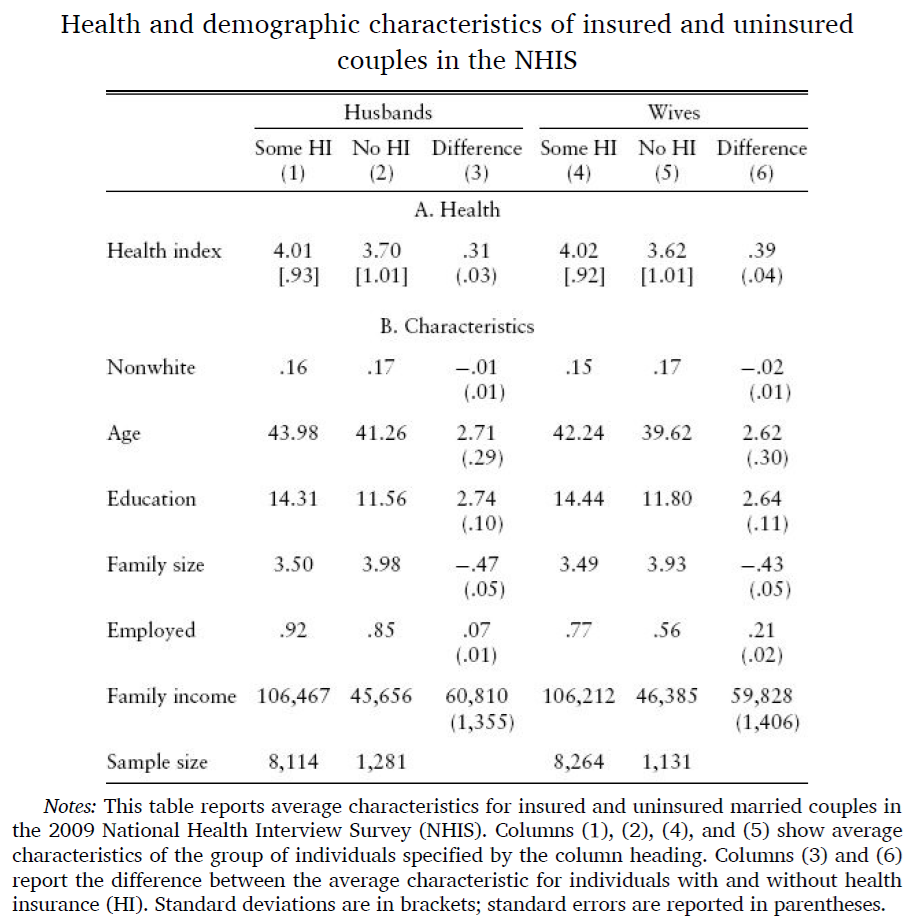
\includegraphics[width=0.6\linewidth]{Table1.png}
\end{figure}

\footnotesize{Source: \textit{Mastering 'Metrics:  The Path from Cause to Effect}, Angrist and Pischke (2015), Table 1.1.}

\end{frame}

\begin{frame}
	\frametitle{Randomized controlled trial (RCT)}
Note that if we assume that \textit{assignment to treatment is random},
\[
\{ Y_i(1), Y_i(0) \} \perp D_i,
\]
then the selection bias becomes zero,
\[
\mathbb{E}[Y_i(0) \mid D_i = 1] - \mathbb{E}[Y_i(0) \mid D_i = 0] = 0,
\]
which means there is no selection bias under random assignment.

Moreover, under random assignment, ATT equals ATE:
\[
\tau = \underbrace{\mathbb{E}[Y_i(1)\mid D_i=1]-\mathbb{E}[Y_i(0)\mid D_i=1]}_{\text{ATT}} 
= \underbrace{\mathbb{E}[Y_i(1)-Y_i(0)]}_{\text{ATE}}.
\]
Consequently,
\begin{equation*}
	\tau=\mathbb{E}[Y_i \mid D_i = 1] - \mathbb{E}[Y_i \mid D_i = 0].
\end{equation*}
\end{frame}

\begin{frame}{Selection Bias}

\begin{itemize}
	\item \textbf{Selection bias:}
	\begin{itemize}
		\item Difference in untreated potential outcomes across groups
	\end{itemize}
\end{itemize}

\begin{center}
\begin{tabular}{lccc}
	\hline
	\textbf{Scenario} & $\mathbb{E}[Y(0)\mid D=1]$ & $\mathbb{E}[Y(0)\mid D=0]$ & \textbf{Bias} \\
	\hline
	Training Program & 80 & 70 & $+10$ \\
	Remedial Education & 60 & 70 & $-10$ \\
	\hline
\end{tabular}
\end{center}

\medskip

\begin{itemize}
	\item Positive bias: treated units would do better anyway
	\item Negative bias: treated units would do worse anyway
\end{itemize}

\end{frame}


\begin{frame}
	\frametitle{Randomized Controlled Trials (RCTs)}

\begin{itemize}
	\item Key feature:
	\begin{itemize}
		\item \textit{Random assignment} to treatment
	\end{itemize}
	
	\medskip
	
	\item Identification requires:
	
	\medskip
	
	\item \textbf{1. Overlap}
	\begin{itemize}
		\item $0 < P(D_i = 1) < 1$
		\item Every unit can be treated or untreated
	\end{itemize}
	
	\medskip
	
	\item \textbf{2. SUTVA (Stable Unit Treatment Value Assumption)}
	\begin{itemize}
		\item \textit{No interference}: outcomes do not depend on others' treatment
		\item \textit{Consistency}: observed outcome matches the realized treatment
	\end{itemize}

\end{itemize}

\end{frame}

\begin{frame}
	\frametitle{Randomized controlled trial (RCT)}
    \begin{itemize}
        \item The causal mechanism can be represented in an RCT using \textit{causal diagrams} \citep{pearl1995causal,pearl2018book}.
        \item \textit{Directed Acyclic Graph (DAG)} is a graphical representation of a set of variables and their assumed causal relationships.
    \end{itemize}

\begin{figure}[h]
	\centering
	\begin{tikzpicture}[->,>=Stealth,shorten >=1pt,node distance=2.5cm,
		thick,main node/.style={circle,draw,minimum size=7mm}]
		\node[main node] (D) {$D$};
		\node[main node] (Y) [right of=D] {$Y$};
		
		\path (D) edge (Y)
		(D) edge (Y);
	\end{tikzpicture}
	\caption{Directed Acyclic Graph (DAG) implied by a Randomized Controlled Trial (RCT).}
	\label{DAG1}
\end{figure} 

\end{frame}

\begin{frame}
	\frametitle{Randomized controlled trial (RCT)}
The counterfactual representation of the DAG, known as the \textit{Single-World Intervention Graph} (SWIG)

\begin{figure}[h]
	\centering
	\begin{tikzpicture}[->,>=Stealth,shorten >=1pt,node distance=2.5cm,
		thick,main node/.style={circle,draw,minimum size=7mm}]
		% Nodes
		\node[main node] (Dfix) {$D = d$};    % Fixed intervention
		\node[main node] (Y) [right of=Dfix] {$Y(d)$}; % Counterfactual outcome
		\node[main node] (Dnat) [below of=Dfix, node distance=1.5cm] {$D$}; % Natural value (irrelevant)
		
		% Edges
		\path (Dfix) edge[dashed] (Y); % Dashed arrow
	\end{tikzpicture}
	\caption{Single-World Intervention Graph (SWIG) for intervention $do(D=d)$: $Y$ is replaced by the counterfactual $Y(d)$, and $D$ is split into the fixed value $D=d$ and its natural value $D$. The dashed arrow indicates the fixed causal assignment.}
	\label{SWIG1}
\end{figure}

\end{frame}

\begin{frame}
	\frametitle{Randomized Controlled Trials (RCTs)}

\begin{itemize}
	\item Observed outcome:
\end{itemize}

\[
Y_i = [Y_i(1) - Y_i(0)] D_i + Y_i(0)
\]

\begin{itemize}
	\item Interpretation:
	\begin{itemize}
		\item Equals $Y_i(0)$ if $D_i=0$
		\item Equals $Y_i(1)$ if $D_i=1$
	\end{itemize}
	
	\medskip
	
	\item Assume:
	\begin{itemize}
		\item Constant treatment effect
		\item Linear CEF: $\mathbb{E}[Y_i \mid D_i]$
	\end{itemize}
	
	\medskip
	
	\item Linear representation \citep{angrist2009mostly}:
\end{itemize}

\[
Y_i = \underbrace{\beta_0}_{\mathbb{E}[Y_i(0)]}
+ \underbrace{\tau}_{\text{treatment effect}} D_i
+ \underbrace{\mu_i}_{Y_i(0) - \mathbb{E}[Y_i(0)]}
\]

\begin{itemize}
	\item $\tau$: common treatment effect
\end{itemize}

\end{frame}

\begin{frame}
	\frametitle{Randomized Controlled Trials (RCTs)}

\begin{itemize}
	\item Under random assignment:
\end{itemize}

\begin{equation*}
	\mathbb{E}[\mu_i \mid D_i] 
	= \mathbb{E}[Y_i(0) \mid D_i] - \mathbb{E}[Y_i(0)] 
	= 0
\end{equation*}

\begin{itemize}
	\item Interpretation:
	\begin{itemize}
		\item Error term is \textit{mean-independent} of treatment
	\end{itemize}
	
	\medskip
	
	\item Implication:
	\begin{itemize}
		\item Regression of $Y_i$ on $D_i$ identifies the causal effect
	\end{itemize}
\end{itemize}

\end{frame}

\begin{frame}
	\frametitle{Student/Teacher Achievement Ratio Experiment}

\begin{itemize}
	\item \textbf{Context STAR experiment:}
	\begin{itemize}
		\item Large-scale randomized experiment (1985--1989)
		\item Cost: $\sim\$12$ million
		\item $\sim$11,600 students (starting in kindergarten)
	\end{itemize}
	
	\medskip
	
	\item \textbf{Objective:}
	\begin{itemize}
		\item Estimate the causal effect of class size on student outcomes
	\end{itemize}
	
	\medskip
	
	\item \textbf{Treatments:}
	\begin{itemize}
		\item Small classes: 13--17 students
		\item Regular classes: 22--25 students
		\item Regular classes + teacher’s aide (part-time or full-time)
	\end{itemize}
	
	\medskip
	
	\item \textbf{Design:}
	\begin{itemize}
		\item Random assignment of students to treatments
		\item Schools participated if $\geq$ 3 classes per grade
		\item Followed students from kindergarten to grade 3
	\end{itemize}

\end{itemize}

\end{frame}

\section{Conditional independence assumption (CIA)}
\begin{frame}
	\frametitle{Conditional Independence Assumption (CIA)}

\begin{itemize}
	\item In RCTs:
	\begin{itemize}
		\item Treatment is assigned randomly
	\end{itemize}
	
	\medskip
	
	\item In observational studies:
	\begin{itemize}
		\item Treatment is determined by choice $\Rightarrow$ potential selection bias
	\end{itemize}
	
	\medskip
	
	\item \textbf{CIA (Unconfoundedness):}
\end{itemize}

\[
\{ Y_i(1), Y_i(0) \} \perp D_i \mid \mathbf{X}_i
\]

\begin{itemize}
	\item Conditional on pre-treatment covariates $\mathbf{X}_i$:
	\begin{itemize}
		\item Treatment assignment is “as good as random”
	\end{itemize}
	
	\medskip
	
	\item \textbf{Overlap (positivity):}
	\begin{itemize}
		\item $0 < P(D_i = 1 \mid \mathbf{X}_i) < 1$
	\end{itemize}
\end{itemize}

\end{frame}

\begin{frame}
	\frametitle{Conditional independence assumption (CIA)}
Note that under the CIA,
\begin{align*}
	\text{ATE} &= \mathbb{E}[Y_i(1)] - \mathbb{E}[Y_i(0)] \\
	&= \mathbb{E}_{\mathbf{X}}\left\{ \mathbb{E}[Y_i(1)\mid \mathbf{X}_i] - \mathbb{E}[Y_i(0)\mid \mathbf{X}_i] \right\} \\
	&= \mathbb{E}_{\mathbf{X}}\left\{ \mathbb{E}[Y_i(1)\mid \mathbf{X}_i, D_i=1] - \mathbb{E}[Y_i(0)\mid \mathbf{X}_i, D_i=0] \right\} \\
	&= \mathbb{E}_{\mathbf{X}}\left\{ \mathbb{E}[Y_i\mid \mathbf{X}_i, D_i=1] - \mathbb{E}[Y_i\mid \mathbf{X}_i, D_i=0] \right\} \\
	&= \mathbb{E}_{\mathbf{X}}\left\{ \tau(\mathbf{X}_i) \right\},
\end{align*}
and
\[
\tau(\mathbf{X}_i) = \mathbb{E}[Y_i \mid \mathbf{X}_i, D_i=1] - \mathbb{E}[Y_i \mid \mathbf{X}_i, D_i=0]
\]
is the \textit{conditional average treatment effect} (CATE) at covariate value $\mathbf{X}_i$, which captures treatment effect heterogeneity across different values of $\mathbf{X}$.
\end{frame}

\begin{frame}
	\frametitle{Conditional independence assumption (CIA)}
Under the CIA, the causal effect of $D$ on $Y$ can be identified by conditioning on $\mathbf{X}$, as this set satisfies the \textit{back-door criterion}.

\medskip

\textbf{Back-door criterion:}
\begin{itemize}
	\item No variable in $\mathbf{X}$ is a descendant of $D$
	\item $\mathbf{X}$ blocks all back-door paths from $D$ to $Y$
\end{itemize}

\medskip

\textbf{Back-door path:}
\begin{itemize}
	\item Any path from $D$ to $Y$ that starts with an arrow pointing into $D$
\end{itemize}
\begin{figure}[h!]
	\centering
	\begin{tikzpicture}[->,>=Stealth,shorten >=1pt,node distance=2.5cm,
		thick,main node/.style={circle,draw,minimum size=7mm}]
		\node[main node] (X) {$\mathbf{X}$};
		\node[main node] (D) [right of=X] {$D$};
		\node[main node] (Y) [right of=D] {$Y$};
		
		\path (X) edge (D)
		(X) edge[bend left=20] (Y)
		(D) edge (Y);
	\end{tikzpicture}
	\caption{Directed Acyclic Graph (DAG) implied by the Conditional Independence Assumption (CIA).}
	\label{DAG2}
\end{figure}

\end{frame}

\begin{frame}
	\frametitle{Conditional Independence Assumption (CIA)}

\begin{itemize}
	\item Extend to multiple regression by including pre-treatment covariates:
\end{itemize}

\begin{align*}
	Y_i = \beta_0 + \tau D_i + \mathbf{X}_i^{\top}\boldsymbol{\beta} + \mu_i
\end{align*}

\begin{itemize}
	\item In RCTs:
	\begin{itemize}
		\item $D_i \perp \mathbf{X}_i$
		\item $\Rightarrow$ identification of $\tau$ is unaffected
	\end{itemize}
	
	\medskip
	
	\item Why include $\mathbf{X}_i$?
	\begin{itemize}
		\item Explains variation in $Y_i$
		\item $\Rightarrow$ improves precision of $\hat{\tau}$
	\end{itemize}
\end{itemize}

\end{frame}

\begin{frame}
	\frametitle{Example: 401(k) Eligibility and Financial Assets}

\begin{itemize}
	\item \textbf{Objective:}
	\begin{itemize}
		\item Estimate the causal effect of 401(k) eligibility (\textit{e401})
		\item Outcome: net financial assets (\textit{net\_tfa})
	\end{itemize}
	
	\medskip
	
	\item \textbf{Identification strategy:}
	\begin{itemize}
		\item Eligibility is \textit{conditionally exogenous}
		\item After controlling for job-related characteristics
	\end{itemize}
	
	\medskip
	
	\item \textbf{Controls ($\mathbf{X}$):}
	\begin{itemize}
		\item Age, income, family size, education
		\item Marital status, two-earner household
		\item Defined benefit pension (\textit{db}), IRA participation (\textit{pira})
		\item Home ownership (\textit{hown})
	\end{itemize}
	
	\medskip
	
	\item \textbf{Key assumption (CIA):}
\end{itemize}

\[
\textit{e401} \;\perp\; \textit{net\_tfa} \;\mid\; \mathbf{X}
\]

\end{frame}

\begin{frame}
	\frametitle{Bad Controls and Collider Bias}

\begin{itemize}
	\item Identification relies on conditioning on $\mathbf{X}$
	
	\medskip
	
	\item \textbf{Warning:} more controls are not always better
	\begin{itemize}
		\item Some variables are \textit{bad controls} \citep{angrist2009mostly}
	\end{itemize}
	
	\medskip
	
	\item \textbf{Collider:}
	\begin{itemize}
		\item A variable caused by two (or more) variables
		\item Example: $D \to C \leftarrow \mathbf{X}$
	\end{itemize}
	
	\medskip
	
	\item \textbf{Key insight:}
	\begin{itemize}
		\item Colliders \textit{block} paths by default
		\item Conditioning on a collider \textit{opens} the path
	\end{itemize}
	
	\medskip
	
	\item \textbf{Implication:}
	\begin{itemize}
		\item Conditioning on $C$ induces a spurious link:
		\[
		D \leftrightarrow \mathbf{X} \rightarrow Y
		\]
		\item $\Rightarrow$ biased estimate of the causal effect
	\end{itemize}

\end{itemize}

\end{frame}

\begin{frame}
	\frametitle{Collider Bias (DAG)}

\begin{figure}[h]
	\centering
	\begin{tikzpicture}[->,>=Stealth,shorten >=1pt,node distance=2.5cm,
		thick,main node/.style={circle,draw,minimum size=7mm}]
		% Nodes
		\node[main node] (X) {$\mathbf{X}$};
		\node[main node] (D) [right of=X] {$D$};
		\node[main node] (Y) [right of=D] {$Y$};
		\node[main node] (C) [below of=Y, node distance=1cm] {$C$}; % Collider
		
		% Edges
		\path (X) edge (D)
		(X) edge[bend left=20] (Y)
		(D) edge (Y)
		(D) edge (C)
		(X) edge (C);
	\end{tikzpicture}
	\caption{Directed Acyclic Graph (DAG): The additional collider $C$ caused by both $D$ and $\mathbf{X}$ would open a path between $D$ and $\mathbf{X}$, inducing bias.}
	\label{DAG3}
\end{figure}

\end{frame}

\begin{frame}
	\frametitle{Conditional independence assumption (CIA): Birth-weight ``paradox", collider bias}
\begin{figure}[h!]
	\centering
	\begin{tikzpicture}[
		node distance=2cm,
		thick,
		main/.style={circle, draw, minimum size=8mm},
		>={Stealth}
		]
		
		% Nodes
		\node[main] (S) {$S$};
		\node[main] (B) [below right=1.2cm and 1.8cm of S] {$B$};
		\node[main, dashed] (U) [below left=1.2cm and 1.8cm of B] {$U$};
		\node[main] (Y) [right=1cm of B] {$Y$};
		
		% Arrows
		\draw[->] (S) -- (B);
		\draw[->] (S) -- (Y);
		\draw[->] (B) -- (Y);
		\draw[->] (U) -- (B);
		\draw[->] (U) -- (Y);
		
	\end{tikzpicture}
	\caption{DAG illustrating the birth-weight paradox: $S$ (smoking), $B$ (birth weight), $Y$ (infant mortality), and $U$ (other unobserved health factors).}
	\label{fig:coll}
\end{figure}	
\end{frame}

\section{Instrumental variables}

\begin{frame}
	\frametitle{Instrumental variables}
\begin{itemize}
	\item \textit{Relevance}, meaning the instruments are correlated with the treatment:
	\[
	\mathbf{Z}_i \not\perp D_i.
	\]
	\item \textit{Exogeneity}, which in the linear model requires:
	\begin{equation*}
		\mathbb{E}[\mu_i \mid \mathbf{Z}_i] = 0,
	\end{equation*}
	and, in terms of potential outcomes, entails:
	\begin{itemize}
		\item \textit{Exclusion restriction}: instruments affect the outcome only through the treatment:
		\begin{align*}
		    Y_i(D_i = d, \mathbf{Z}_i = \mathbf{z}) & = Y_i(D_i = d, \mathbf{Z}_i = \mathbf{z}') = Y_i(D_i = d),\\
            &d \in \{0,1\},
		\end{align*}
			
		\item \textit{Marginal exchangeability}: instruments are independent of the potential outcomes:
		\[
		\mathbf{Z}_i \perp \{ Y_i(1), Y_i(0) \}.
		\]
	\end{itemize}
\end{itemize}

\end{frame}

\begin{frame}
	\frametitle{Instrumental Variables: Monotonicity}

\begin{itemize}
	\item Instrument validity conditions alone imply \textit{partial identification} of LATE
	\begin{itemize}
		\item See \citep{Manski1989,manski1990nonparametric,manski1995identification,manski2003partial}
	\end{itemize}
	
	\medskip
	
	\item To achieve \textbf{point identification}, we impose:
	
	\medskip
	
	\item \textbf{Monotonicity}
	\begin{itemize}
		\item The instrument shifts treatment decisions in the same direction for all units
	\end{itemize}
\end{itemize}

\[
D_i(1) \geq D_i(0), \quad i = 1,\dots,N
\]

\begin{itemize}
	\item (No “defiers” when $Z_i \in \{0,1\}$)
\end{itemize}

\end{frame}
\begin{frame}
	\frametitle{Instrumental variables}
\begin{figure}[h]
	\centering
	\begin{tikzpicture}[->,>=Stealth,shorten >=1pt,node distance=2.5cm,
		thick,main node/.style={circle,draw,minimum size=7mm}]
		% Nodes
		\node[main node, dashed] (U) {$\mathbf{U}$};
		\node[main node] (D) [right of=X] {$D$};
		\node[main node] (Y) [right of=D] {$Y$};
		\node[main node] (Z) [below of=D, node distance=2cm] {$Z$};
		
		% Edges
		\path (Z) edge (D)
		(U) edge[bend left=20] (Y)
		(D) edge (Y)
		(U) edge (D);
	\end{tikzpicture}
	\caption{Directed Acyclic Graph (DAG) showing an instrumental variable $Z$ used to identify the causal effect of $D$ on $Y$ when some confounders $\mathbf{U}$ (dashed) are unobserved or measured with error.}
	\label{DAG4}
\end{figure}
\end{frame}

\begin{frame}
	\frametitle{Instrumental variables}
    {\small{
\begin{table}[ht]
	\centering
	\caption{Distribution of compliance types by instrument and treatment}\label{tab:2x2}
	\begin{tabular}{lcc}
		\hline
		& \multicolumn{2}{c}{\textbf{Treatment}} \\ 
		\cline{2-3}
		\textbf{Instrument} & $D_i = 0$ & $D_i = 1$ \\ 
		\hline
		$Z_i=0$  & Compliers, Never-takers & Always-takers \\[0.25em]
		$Z_i=1$  & Never-takers & Compliers, Always-takers \\ 
		\hline
	\end{tabular}
\end{table}
}}
\end{frame}

\begin{frame}
	\frametitle{Instrumental variables}
\begin{align*}
	\tau_{LATE} 
	&= \mathbb{E}[Y_i(1)-Y_i(0)\mid D_i(1)=1, D_i(0)=0]\\
    &=\frac{\mathbb{E}[Y_i \mid Z_i = 1] - \mathbb{E}[Y_i \mid Z_i = 0]}{\mathbb{E}[D_i \mid Z_i = 1] - \mathbb{E}[D_i \mid Z_i = 0]}.
\end{align*}

\begin{itemize}
	\item The IV estimand is:
	\begin{itemize}
		\item Ratio of the effect of $Z$ on $Y$ (reduced form)
		\item To the effect of $Z$ on $D$ (first stage)
	\end{itemize}
	
	\medskip
	
	\item Interpretation:
	\begin{itemize}
		\item Numerator: how outcomes respond to the instrument
		\item Denominator: how treatment responds to the instrument
	\end{itemize}
	
	\medskip
	
	\item Key insight:
	\begin{itemize}
		\item The instrument induces exogenous variation in $D$
		\item $\Rightarrow$ isolates the causal effect for \textit{compliers}
	\end{itemize}
\end{itemize}
\end{frame}

\begin{frame}
	\frametitle{Instrumental variables: A simple setting for point and set identified LATE}
\begin{table}[ht]
	\centering
	\caption{Distribution of units by type, instrument, treatment, and outcomes}
	\label{tab:types}
	\begin{tabular}{lcccc}
		\hline
		Type & $Z_{obs}$ & $D_{obs}$ & $Y_{obs}$ & Units \\
		\hline
		Compliers, Never-takers & 0 & 0 & 3 & 50 \\
		Never-takers   & 1 & 0 & 4 & 20  \\
		Compliers, Always-takers & 1 & 1 & 7 & 100  \\
		 Always-takers   & 0 & 1 & 5 & 30  \\
		\hline
	\end{tabular}
\end{table}
\end{frame}

\begin{frame}
	\frametitle{Example: 401(k) Participation and Financial Assets}

\begin{itemize}
	\item \textbf{Objective:}
	\begin{itemize}
		\item Estimate the causal effect of 401(k) participation (\textit{p401})
		\item Outcome: net financial assets (\textit{net\_tfa})
	\end{itemize}

	
	\item \textbf{Endogeneity concern:}
	\begin{itemize}
		\item Participation in a 401(k) plan is not random. Individuals who participate may differ systematically in saving preferences
	\end{itemize}

	\item \textbf{Instrument:} eligibility for a 401(k) plan (\textit{e401})

	\item \textbf{Controls ($\mathbf{X}$):}
	\begin{itemize}
		\item Age, income, family size, education, home ownership (\textit{hown}), marital status, two-earner household, defined benefit pension (\textit{db}), IRA participation (\textit{pira})
	\end{itemize}
	
	\item \textbf{IV assumptions:}
	\begin{itemize}
		\item \textit{Relevance:} \textit{e401} affects 401(k) participation
		\item \textit{Exogeneity:} \textit{e401} affects net financial assets only through participation
	\end{itemize}
\end{itemize}

\end{frame}
\section{Difference-in-differences design (DiD)}
\begin{frame}
	\frametitle{Difference-in-Differences ($2 \times 2$)}

\begin{itemize}
	\item Setup:
	\begin{itemize}
		\item Two periods: $t = 1$ (pre), $t = 2$ (post)
		\item Two groups:
		\begin{itemize}
			\item Treated: $D_i = 1$ (treated between $t=1$ and $t=2$)
			\item Control: $D_i = 0$ (never treated)
		\end{itemize}
	\end{itemize}
	
	\medskip
	
	\item Data:
	\begin{itemize}
		\item Outcomes $Y_{it}$ for $i = 1,\dots,N$
		\item Balanced panel
	\end{itemize}
	
	\medskip
	
	\item Potential outcomes:
	\begin{itemize}
		\item $Y_{it}(1)$: treated in period $2$
		\item $Y_{it}(0)$: never treated
	\end{itemize}
	
	\medskip
	
	\item \textbf{Target parameter (ATT):}
\end{itemize}

\[
\tau_{2} = \mathbb{E}\big[ Y_{i2}(1) - Y_{i2}(0) \mid D_i = 1 \big]
\]

\end{frame}

\begin{frame}
	\frametitle{Difference-in-Differences ($2 \times 2$)}
    \begin{itemize}
        \item \textit{Parallel trends:}
\begin{equation*}
	\mathbb{E}[Y_{i2}(0) - Y_{i1}(0) \mid D_i = 1] = \mathbb{E}[Y_{i2}(0) - Y_{i1}(0) \mid D_i = 0],
\end{equation*}
which states that, in the absence of treatment, the average change in outcomes for the treated and control groups would have evolved similarly over time.

\item \textit{No anticipation effects:}
\begin{equation*}
	\mathbb{E}[Y_{i1}(0)\mid D_i=1] = \mathbb{E}[Y_{i1}(1)\mid D_i=1],
\end{equation*}
meaning that the treatment has no causal effect prior to its implementation.
    \end{itemize}
\end{frame}

\begin{frame}
	\frametitle{Difference-in-Differences ($2 \times 2$)}

\begin{figure}[ht]
	\centering
	\begin{tikzpicture}
		\begin{axis}[
			width=10cm,height=7cm,
			xmin=-0.6, xmax=1.5, ymin=0.3, ymax=1.3,
			axis lines=left,
			grid=both, grid style={gray!20},
			xlabel={},
			ylabel={Outcome ($Y_{it}$)},
			xtick={0.2, 1}, xticklabels={$t=1$, $t=2$},
			ytick={0.5, 0.7, 1, 1.2},
			clip=false
			]
			% Sharp RD step:
			\addplot[dashed] coordinates {(-0.6,0.5) (1,0.5)};
			\addplot[dashed] coordinates {(-0.6,0.7) (0.2,0.7)};
			
			\addplot[black, very thick] coordinates {(0.2,0.7) (1,0.6)};
			\addplot[dashed] coordinates {(0.2,0.7) (1,0.5)};
			\draw[<->] (axis cs:0.2,0.7) -- (axis cs:0.2,0.5);
			\node[red] at (axis cs:-0.2,0.65) {\tiny Parallel trends};
			\node[black] at (axis cs:-0.2,0.6) {\tiny $\mathbb{E}[Y_{i2}(0) - Y_{i1}(0) \mid D_i = 1] = $};
			\node[blue] at (axis cs:-0.2,0.55) {\tiny $ \mathbb{E}[Y_{i2}(0) - Y_{i1}(0) \mid D_i = 0]$};
			
			\addplot[dashed] coordinates {(-0.6,1) (1,1)};
			\addplot[dashed] coordinates {(-0.6,1.2) (0.2,1.2)};
			
			\addplot[black, very thick] coordinates {(0.2,1.2) (1,1)};
			\draw[<->] (axis cs:0.2,1.2) -- (axis cs:0.2,1);
			\node[blue] at (axis cs:-0.2,1.1) {\tiny $\mathbb{E}[Y_{i2}(0) - Y_{i1}(0) \mid D_i = 0]$};
			\node[black] at (axis cs:0.2,1.22) {\tiny $\mathbb{E}[Y_{i1}(0) \mid D_i = 0]$};
			\node[black] at (axis cs:1.25,1.02) {\tiny $\mathbb{E}[Y_{i2}(0) \mid D_i = 0]$};
			\node[red] at (axis cs:0.2,0.72) {\tiny No anticipation: $\mathbb{E}[Y_{i1}(1) \mid D_i = 1]=\mathbb{E}[Y_{i1}(0) \mid D_i = 1]$};
			\node[black] at (axis cs:1.22,0.62) {\tiny $\mathbb{E}[Y_{i2}(1) \mid D_i = 1]$};
			\draw[<->, red] (axis cs:1,0.6) -- (axis cs:1,0.5);
			\node[red] at (axis cs:1.4,0.555) {\tiny $ATT=\mathbb{E}[Y_{i2}(1) \mid D_i = 1]-$};
			\node[red] at (axis cs:1.482,0.525) {\tiny $\mathbb{E}[Y_{i2}(0) \mid D_i = 1]$};
			\node[red] at (axis cs:0.6,0.47) {\tiny $\mathbb{E}[Y_{i2}(0) \mid D_i = 1]=\mathbb{E}[Y_{i1} \mid D_i = 1] + \mathbb{E}[Y_{i2} - Y_{i1} \mid D_i = 0]$};
			
			\fill[black] (axis cs:0.2,1.2) circle (2pt);
			\fill[black] (axis cs:1,1) circle (2pt);
			\fill[black] (axis cs:0.2,0.7) circle (2pt);
			\fill[black] (axis cs:1,0.6) circle (2pt);
			\fill[red] (axis cs:1,0.5) circle (2pt);
			%\draw[black, fill=black] (0.7,1) circle (2pt);
			%\draw[black, fill=black] (0.2,0.7) circle (2pt);
			%\draw[black, fill=black] (0.7,0.6) circle (2pt);
			% Cutoff (vertical dashed line)
			%\addplot[black, densely dashed, very thick] coordinates {(0,0) (0,1.02)};
			
			% Labels
			%\node[black] at (axis cs:-0.52,0.92) {\large Assigned to Control};
			%\node[black]  at (axis cs: 0.52,0.92) {\large Assigned to Treatment};
			
			% Arrow and text to mark "Cutoff"
			%\draw[->] (axis cs:0.28,0.2) -- (axis cs:0.02,0.2);
			%\node[anchor=west] at (axis cs:0.3,0.2) {Cutoff};
			
			% Bracket showing jump size (optional)
			%\draw[<->, thick] (axis cs:0.04,0.0) -- (axis cs:0.04,1);
			%\node[anchor=west] at (axis cs:0.06,0.50) {$\Delta P$};
		\end{axis}
	\end{tikzpicture}
	%\caption{Difference-in-Differences: Identification strategy}
	\label{Fig:DiD}
\end{figure}

\end{frame}

\begin{frame}
	\frametitle{Difference-in-Differences ($2 \times 2$)}
The ATT is the difference in outcome differences between treated and control units,
\begin{equation}\label{eq:DiD}
\tau_2 = \mathbb{E}[Y_{i2} - Y_{i1} \mid D_i = 1] - \mathbb{E}[Y_{i2} - Y_{i1} \mid D_i = 0],
\end{equation}

\end{frame}

\begin{frame}
	\frametitle{Difference-in-Differences ($2 \times 2$)}
En regression forms:
\[
Y_{it} = \alpha_i + \phi_t + \tau_2 D_i + \mu_{it},
\]
which implies
\[
Y_{i2} - Y_{i1} = (\phi_2 - \phi_1) + \tau_2 D_i + (\mu_{i2} - \mu_{i1}).
\]
The two-way fixed effects (TWFE) model
\[
Y_{it} = \alpha + \alpha_i + \phi_t + \tau_2 \,\big[ D_i \cdot \mathbbm{1}(t = 2) \big] + \epsilon_{it},
\]
where $\mathbbm{1}(t = 2)$ is an indicator for the post-treatment period \citep{roth2023whats}.
\end{frame}

\begin{frame}
	\frametitle{Difference-in-Differences ($2 \times 2$)}

\begin{itemize}
	\item Extension: condition on covariates $\mathbf{X}$
	\begin{itemize}
		\item Compare units that are similar in observed characteristics
		\item Identification assumptions hold \textit{conditional on} $\mathbf{X}$
	\end{itemize}
	
	\medskip
	
	\item Estimation:
	\begin{itemize}
		\item Linear regression (parametric)
	\end{itemize}
	
	\medskip
	
	\item Alternatives (more flexible):
	\begin{itemize}
		\item \textit{Outcome regression} (OR)
		\item \textit{Inverse probability weighting} (IPW)
		\item \textit{Doubly robust} (OR + IPW)
	\end{itemize}
	
	\medskip
	
	\item Key advantage:
	\begin{itemize}
		\item Consistent under conditional parallel trends
		\item No need to assume a linear CEF
	\end{itemize}
\end{itemize}

\end{frame}

\begin{frame}
	\frametitle{Difference-in-Differences ($2 \times 2$): Assumptions}

\begin{itemize}
	\item \textbf{Functional form matters:}
	\begin{itemize}
		\item Parallel trends may not be preserved under transformations of $Y$
	\end{itemize}
	
	\medskip
	
	\item \textbf{Limitations:}
	\begin{itemize}
		\item Parallel trends and no anticipation are \textit{not testable}
		\item They involve counterfactual outcomes we do not observe
	\end{itemize}
	
	\medskip
	
	\item \textbf{What can we do?}
	\begin{itemize}
		\item Examine pre-treatment trends
		\item Assess plausibility of the identifying assumptions
	\end{itemize}
\end{itemize}
\end{frame}

\begin{frame}
	\frametitle{Staggered DiD (Multiple Periods)}

\begin{itemize}
	\item Many applications go beyond the \(2 \times 2\) design
	
	\medskip
	
	\item Key idea:
	\begin{itemize}
		\item Staggered DiD is an aggregation of multiple \(2 \times 2\) comparisons
		\item Compare treated units with \textit{not-yet-treated} units \citep{baker2025did_guide}
	\end{itemize}
	
	\medskip
	
	\item \textbf{Setup:}
	\begin{itemize}
		\item Periods: \(t = 1, \dots, T\)
		\item Treatment is \textit{absorbing}: once treated, always treated
	\end{itemize}
\end{itemize}

\medskip

\[
G_i = \min\{t : D_{it} = 1\}
\]

\begin{itemize}
	\item \(G_i\): first period in which unit \(i\) is treated
\end{itemize}

\end{frame}

\begin{frame}
	\frametitle{Staggered DiD (Multiple Periods)}

\begin{itemize}
	\item \textbf{Potential outcomes:}
	\begin{itemize}
		\item \(Y_{it}(g)\): outcome for a unit first treated in period \(g\)
		\item \(Y_{it}(\infty)\): outcome for a never-treated unit
	\end{itemize}
\end{itemize}

\medskip

\[
ATT(g,t) = \mathbb{E}\big[ Y_{it}(g) - Y_{it}(\infty) \mid G_i = g \big]
\]

\begin{itemize}
	\item \(ATT(g,t)\): average treatment effect for units first treated in period \(g\), evaluated at time \(t\)
	
	\medskip
	
	\item Each cohort \(g\) has its own treatment effects over time
\end{itemize}

\end{frame}

\begin{frame}
	\frametitle{Staggered DiD: Identifying Assumptions}

\begin{itemize}
	\item \textbf{1. Staggered parallel trends (not-yet-treated):}
\end{itemize}

\begin{equation*}
\mathbb{E}[Y_{it}(\infty) - Y_{it-1}(\infty) \mid G_i = g] 
= \mathbb{E}[Y_{it}(\infty) - Y_{it-1}(\infty) \mid G_i = g'], 
\quad \forall\, t \geq g,\; g' > t
\end{equation*}

\begin{itemize}
	\item Interpretation:
	\begin{itemize}
		\item In the absence of treatment, groups would evolve in parallel
		\item Comparison group: \textit{not-yet-treated} units
	\end{itemize}
	
	\medskip
	
	\item Alternative comparison groups:
	\begin{itemize}
		\item \textit{Never-treated}: $g' = \infty$
		\item \textit{All groups}: parallel trends across all $g, g'$
	\end{itemize}
\end{itemize}

\end{frame}

\begin{frame}
	\frametitle{Staggered DiD: Additional Assumptions}

\begin{itemize}
	\item \textbf{2. No anticipation:}
\end{itemize}

\begin{equation*}
\mathbb{E}[Y_{it}(g)] = \mathbb{E}[Y_{it}(\infty)], 
\quad \forall\, t < g
\end{equation*}

\begin{itemize}
	\item Units do not change behavior before treatment
	
	\medskip
	
	\item \textbf{Trade-offs across assumptions:}
	\begin{itemize}
		\item \textit{All groups}: stronger assumption, more precision
		\item \textit{Never-treated}: weaker assumption, less precision
		\item \textit{Not-yet-treated}: intermediate case
	\end{itemize}
	
	\medskip
	
	\item \textbf{Implication:}
	\begin{itemize}
		\item Long-run effects: require parallel trends after treatment
		\item Short-run effects: require parallel trends in the relevant period
	\end{itemize}
\end{itemize}

\end{frame}

\begin{frame}
	\frametitle{Staggered DiD: Identification and Dynamics}

\begin{itemize}
	\item Under the identifying assumptions, $ATT(g,t)$ can be written as:
\end{itemize}
\begin{align*}
ATT(g,t) 
= \mathbb{E}\big[ Y_{it} - Y_{i,g-1} \mid G_i = g \big]
- \mathbb{E}\big[ Y_{it} - Y_{i,g-1} \mid G_i = g' \big], \quad g' > t
\end{align*}

\begin{itemize}
	\item Interpretation:
	\begin{itemize}
		\item Change in outcomes for cohort $g$
		\item Relative to a comparison group (not-yet-treated or never-treated)
	\end{itemize}
	
	\item Key features:
	\begin{itemize}
		\item Cohorts indexed by first treatment period $g$
		\item Effects evaluated at time $t$
		\item $\Rightarrow$ multiple cohort--time effects $ATT(g,t)$
	\end{itemize}
	
	\item \textbf{Dynamics:}
	\begin{itemize}
		\item Use \textit{event-study} plots
		\item Track effects before and after treatment
	\end{itemize}
\end{itemize}

\end{frame}

\begin{frame}
	\frametitle{Staggered DiD: Placebo Tests}

\begin{itemize}
	\item Advantage of multiple pre-treatment periods:
	\begin{itemize}
		\item Enables \textit{placebo (falsification) tests}
	\end{itemize}
	
	\medskip
	
	\item Under \textbf{no anticipation}:
	\begin{itemize}
		\item Treatment has no effect before it occurs
	\end{itemize}
\end{itemize}
\[
\mathbb{E}\!\left[Y_{it} - Y_{ib} \mid G_i = g\right]
=
\mathbb{E}\!\left[Y_{it} - Y_{ib} \mid G_i = g'\right],
\ b < t < \min\{g,g'\}
\]

\begin{itemize}
	\item \textbf{Test:}
	\begin{itemize}
		\item Pre-treatment differences should be statistically zero
	\end{itemize}
	
	\medskip
	
	\item \textbf{Interpretation:}
	\begin{itemize}
		\item Supports (but does not prove) parallel trends
	\end{itemize}
	
	\medskip
	
	\item \textbf{Caution:}
	\begin{itemize}
		\item Parallel trends is fundamentally \textit{untestable}
		\item Requires sensitivity analysis
	\end{itemize}
\end{itemize}

\end{frame}

\begin{frame}
	\frametitle{Staggered DiD with Covariates}

\begin{itemize}
	\item Assume parallel trends holds \textit{conditional on} $\mathbf{X}_i$
	
	\medskip
	
	\item \textbf{1. Conditional parallel trends (not-yet-treated):}
\end{itemize}
{\footnotesize{
\begin{align*}
\mathbb{E}\!\left[Y_{it}(\infty)-Y_{i,t-1}(\infty)\mid G_i=g,\mathbf{X}_i\right]
=
\mathbb{E}\!\left[Y_{it}(\infty)-Y_{i,t-1}(\infty)\mid G_i=g',\mathbf{X}_i\right],
\\
\ t \geq g,\; g' > t
\end{align*}
}}
\begin{itemize}
	\item \textbf{2. Overlap (positivity):}
\end{itemize}
\[
P(G_i = g \mid \mathbf{X}_i) < 1 - \epsilon, \quad \epsilon > 0, \quad P(G_i = g) > 0
\]

\begin{itemize}
	\item Interpretation:
	\begin{itemize}
		\item Comparable units exist across cohorts given $\mathbf{X}_i$
	\end{itemize}
\end{itemize}

\end{frame}

\begin{frame}
	\frametitle{Staggered DiD with Covariates}

\begin{itemize}
	\item Under these assumptions (and no anticipation):
\end{itemize}
\begin{align*}
ATT(g,t) 
&= \mathbb{E}[Y_{it} - Y_{i,g-1} \mid G_i = g] \\
&\quad - \mathbb{E}_{\mathbf{X}}\!\left\{
\mathbb{E}[Y_{it} - Y_{i,g-1} \mid \mathbf{X}_i, G_i = g'] 
\mid G_i = g
\right\}
\end{align*}

\begin{itemize}
	\item \textbf{Estimation:}
	\begin{itemize}
		\item Outcome regression (OR)
		\item Inverse probability weighting (IPW)
		\item Doubly robust methods
	\end{itemize}
	
	\medskip
	
	\item \textbf{Caution:}
	\begin{itemize}
		\item TWFE does \textit{not} generally identify $ATT(g,t)$
		\item Can produce non-convex weights (even negative)
	\end{itemize}
\end{itemize}

\end{frame}

\begin{frame}
	\frametitle{Application: Minimum Wage and Teen Employment \citep{callaway2021difference}}

\begin{itemize}
	\item \textbf{Context:}
	\begin{itemize}
		\item Period: 2001--2007 (federal minimum wage fixed at \$5.15)
		\item Outcome: county-level teen employment
	\end{itemize}
	
	\medskip
	
	\item \textbf{Treatment definition:}
	\begin{itemize}
		\item States that increased minimum wage $\Rightarrow$ treated
		\item Groups defined by first year of increase (staggered adoption)
		\item States with no increase $\Rightarrow$ control group
	\end{itemize}
	
	\medskip
	
	\item \textbf{Why this design?}
	\begin{itemize}
		\item More variation than local case studies
		\item Clean identification from state-level policy changes
	\end{itemize}
\end{itemize}

\end{frame}

\begin{frame}
	\frametitle{Application: Data and Empirical Features}

\begin{itemize}
	\item \textbf{Data:}
	\begin{itemize}
		\item Teen employment: Quarterly Workforce Indicators (QWI)
		\item County characteristics:
		\begin{itemize}
			\item Population, race, education
			\item Income and poverty measures
		\end{itemize}
	\end{itemize}
	
	\medskip
	
	\item \textbf{Sample:}
	\begin{itemize}
		\item 29 states after exclusions
	\end{itemize}
	
	\medskip
	
	\item \textbf{Empirical advantages:}
	\begin{itemize}
		\item Enables staggered DiD estimation
		\item Allows testing of pre-treatment trends
		\item Supports event-study analysis
	\end{itemize}
\end{itemize}

\end{frame}

\section{Regression discontinuity design (RD)}

\begin{frame}
	\frametitle{Regression Discontinuity Design (RD)}

\begin{itemize}
	\item \textbf{Key ingredient:} running variable $Z_i$
	\begin{itemize}
		\item Also called forcing, index, or score variable
		\item Determines treatment assignment relative to cutoff $c$
	\end{itemize}
	
	\medskip
	
	\item \textbf{Identification idea:}
	\begin{itemize}
		\item Potential outcomes vary \textit{smoothly} in $Z_i$
		\item Any discontinuity at $c$ is attributed to treatment
	\end{itemize}
	
	\medskip
	
	\item \textbf{Treatment jump at the cutoff:}
\end{itemize}

\begin{align*}
\Delta &= \lim_{z \downarrow c}\Pr(D_i=1 \mid Z_i=z)
- \lim_{z \uparrow c}\Pr(D_i=1 \mid Z_i=z)
\\
&=
\begin{cases}
1, & \text{sharp RD},\\
\in (0,1), & \text{fuzzy RD}
\end{cases}
\end{align*}

\begin{itemize}
	\item Right and left limits: approach $c$ from above and below
\end{itemize}

\end{frame}
\begin{frame}
	\frametitle{Regression discontinuity design (RD): Sharp}
\[
D_i = \mathbbm{1}\{Z_i \ge c\},
\]
\begin{figure}[ht]
	\centering
	\begin{tikzpicture}
		\begin{axis}[
			width=10cm,height=5.5cm,
			xmin=-1, xmax=1, ymin=0, ymax=1.05,
			axis lines=left,
			grid=both, grid style={gray!20},
			xlabel={Running variable ($Z$)},
			ylabel={\small{Conditional probability of treatment}},
			xtick={0}, xticklabels={$c$},
			ytick={0,0.5,1},
			clip=false
			]
			% Sharp RD step:
			\addplot[very thick] coordinates {(-1,0) (0,0)};
			\addplot[very thick]  coordinates {(0,1) (1,1)};
			
			% Cutoff (vertical dashed line)
			\addplot[black, densely dashed, very thick] coordinates {(0,0) (0,1.02)};
			
			% Labels
			\node[black] at (axis cs:-0.52,0.92) {\small Assigned to Control};
			\node[black]  at (axis cs: 0.52,0.92) {\small Assigned to Treatment};
			
			% Arrow and text to mark "Cutoff"
			\draw[->] (axis cs:0.28,0.2) -- (axis cs:0.02,0.2);
			\node[anchor=west] at (axis cs:0.3,0.2) {Cutoff};
			
			% Bracket showing jump size (optional)
			\draw[<->, thick] (axis cs:0.04,0.0) -- (axis cs:0.04,1);
			\node[anchor=west] at (axis cs:0.06,0.50) {$\Delta P$};
		\end{axis}
	\end{tikzpicture}
\caption{Sharp regression discontinuity design: Conditional probability of treatment}
\label{Fig:SRDD}
\end{figure}

\end{frame}


\begin{frame}
	\frametitle{Regression discontinuity design (RD): Sharp}
\[
\tau_{\text{SRD}}
= \lim_{z \downarrow c}\mathbb{E}[Y_i\mid Z_i=z]
- \lim_{z \uparrow c}\mathbb{E}[Y_i\mid Z_i=z],
\]
\begin{figure}[ht]
	\centering
	\begin{tikzpicture}
		\begin{axis}[
			width=10cm,height=6cm,
			xmin=-1, xmax=1, ymin=0, ymax=1.05,
			axis lines=left,
			grid=both, grid style={gray!20},
			xlabel={Running variable ($Z$)},
			ylabel={$\mathbb{E}[Y(1)\mid Z],\ \mathbb{E}[Y(0)\mid Z]$},
			xtick={0}, xticklabels={$c$},
			ytick=\empty,
			clip=false
			]
			
			% --- Choose smooth functions for illustration ---
			% E[Y(0)|X]: observed (solid) for X<c, counterfactual (dashed) for X>=c
			\addplot[black, very thick, domain=-1:0, samples=200] {0.35 + 0.1*x + 0.05*x^2};
			\addplot[black, very thick, dashed, domain=0:1, samples=200] {0.35 + 0.1*x + 0.05*x^2};
			
			% E[Y(1)|X]: counterfactual (dashed) for X<c, observed (solid) for X>=c
			\addplot[black, very thick, dashed, domain=-1:0, samples=200] {0.62 + 0.06*x + 0.08*x^2};
			\addplot[black, very thick, domain=0:1, samples=200] {0.62 + 0.06*x + 0.08*x^2};
			
			% --- Cutoff (vertical dashed line) ---
			\addplot[black, densely dashed, very thick] coordinates {(0,0) (0,1.02)};
			
			% --- Points at the cutoff (mu_- and mu_+) ---
			\filldraw[black] (axis cs:0,0.35) circle (2pt);  % mu_-
			\filldraw[black] (axis cs:0,0.62) circle (2pt);  % mu_+
			
			% Labels mu_- and mu_+
			% \node[anchor=east] at (axis cs:-0.02,0.35) {$\mu_-$};
			% \node[anchor=east] at (axis cs:-0.02,0.62) {$\mu_+$};
			
			% --- Jump size tau_SRD ---
			\draw[<->, thick] (axis cs:0.06,0.35) -- (axis cs:0.06,0.62);
			\node[anchor=west] at (axis cs:0.07,0.485) {$\tau_{\text{SRD}}$};
			
			% --- Arrow + label "Cutoff" ---
			\draw[->] (axis cs:0.28,0.08) -- (axis cs:0.02,0.08);
			\node[anchor=west] at (axis cs:0.30,0.08) {Cutoff};
			
			% --- Curve labels ---
			\node[black, anchor=west]  at (axis cs:0.45,0.80) {$\mathbb{E}[Y(1)\mid Z]$};
			\node[black, anchor=west] at (axis cs:0.45,0.30) {$\mathbb{E}[Y(0)\mid Z]$};
			
		\end{axis}
	\end{tikzpicture}
	\caption{RD treatment effect in a sharp RD design. Solid segments are observed on each side of $c$; dashed segments are counterfactual \cite{cattaneo2019practical}.}
	\label{fig:SRD-muplus-muminus}
\end{figure}

\end{frame}

\begin{frame}
	\frametitle{Regression discontinuity design (RD): Fuzzy}
    \begin{align*}
	0 \;<\; \lim_{z \downarrow c} \Pr(D_i=1 \mid Z_i=z) \;-\; \lim_{z \uparrow c} \Pr(D_i=1 \mid Z_i=z) \;<\; 1.
\end{align*}
\begin{figure}[ht]
	\centering
	\begin{tikzpicture}
		\begin{axis}[
			width=8cm,height=5.5cm,
			xmin=-1, xmax=1, ymin=0, ymax=1.05,
			axis lines=left,
			grid=both, grid style={gray!20},
			xlabel={Running variable ($Z$)},
			ylabel={\footnotesize Conditional probability of treatment},
			xtick={0}, xticklabels={$c$},
			ytick={0,0.5,1},
			clip=false
			]
			% Fuzzy RD: probabilities below/above cutoff
			\addplot[very thick] coordinates {(-1,0.20) (0,0.30)};  % left limit p^-
			\addplot[very thick] coordinates {(0,0.80) (1,0.90)};   % right limit p^+
			
			% Open circles at the jump (left/right limits at c)
			\draw[thick, fill=white] (axis cs:0,0.30) circle (2.2pt);
			\draw[thick, fill=white] (axis cs:0,0.80) circle (2.2pt);
			
			% Cutoff (vertical dashed line)
			\addplot[black, densely dashed, very thick] coordinates {(0,0) (0,1.02)};
			
			% Labels for regions
			\node[black] at (axis cs:-0.52,0.92) {\footnotesize Assigned to Control};
			\node[black] at (axis cs: 0.52,0.92) {\footnotesize Assigned to Treatment};
			
			% Arrow and text to mark "Cutoff"
			\draw[->] (axis cs:0.28,0.12) -- (axis cs:0.02,0.12);
			\node[anchor=west] at (axis cs:0.30,0.12) {Cutoff};
			
			% Bracket showing jump size (optional)
			\draw[<->, thick] (axis cs:0.04,0.30) -- (axis cs:0.04,0.80);
			\node[anchor=west] at (axis cs:0.06,0.50) {$\Delta P$};
			
		\end{axis}
	\end{tikzpicture}
	\caption{Fuzzy regression discontinuity design: Conditional probability of treatment}
	\label{Fig:FRDD}
\end{figure}
\end{frame}

\begin{frame}
	\frametitle{Regression discontinuity design (RD): Fuzzy}
The identification assumptions are: 

\textit{1. Continuity of the potential outcome regression functions}, particularly at \(c\).

\textit{2. A nontrivial first stage},
\(\lim_{z \downarrow c}\mathbb{E}[D_i\mid Z_i=z]-\lim_{z \uparrow c}\mathbb{E}[D_i\mid Z_i=z]\neq 0\),

and 

\textit{3. Monotonicity}: \(D_i(z)\) is non-increasing in \(z\) at \(z=c\).

\end{frame}

\begin{frame}
	\frametitle{Regression discontinuity design (RD): Fuzzy}
\begin{align*}
\tau_{\text{FRD}}
&=
\frac{\lim_{z \downarrow c}\mathbb{E}[Y_i\mid Z_i=z]-\lim_{z \uparrow c}\mathbb{E}[Y_i\mid Z_i=z]}
{\lim_{z \downarrow c}\mathbb{E}[D_i\mid Z_i=z]-\lim_{z \uparrow c}\mathbb{E}[D_i\mid Z_i=z]}.
\end{align*}

\begin{figure}[ht]
	\centering
	\begin{tikzpicture}
		\begin{axis}[
			width=10cm,height=6cm,
			xmin=-1, xmax=1, ymin=0, ymax=1.05,
			axis lines=left,
			grid=both, grid style={gray!20},
			xlabel={Running variable ($Z$)},
			ylabel={$\mathbb{E}[Y\mid Z]$},
			xtick={0}, xticklabels={$c$},
			ytick=\empty,
			clip=false
			]
			
			% --- Choose smooth functions for illustration ---
			% E[Y(0)|X]: observed (solid) for X<c, counterfactual (dashed) for X>=c
			\addplot[black, very thick, dashed, domain=-1:0, samples=200] {0.35 + 0.1*x + 0.05*x^2};
			\addplot[black, very thick, dashed, domain=0:1, samples=200] {0.35 + 0.1*x + 0.05*x^2};
			
			% E[Y(1)|X]: counterfactual (dashed) for X<c, observed (solid) for X>=c
			\addplot[black, very thick, dashed, domain=-1:0, samples=200] {0.62 + 0.06*x + 0.08*x^2};
			\addplot[black, very thick, dashed, domain=0:1, samples=200] {0.62 + 0.06*x + 0.08*x^2};
			
			% E[Y(1)|X]: counterfactual (dashed) for X<c, observed (solid) for X>=c
			\addplot[black, very thick, domain=-1:0, samples=200] {0.4 + 0.09*x + 0.06*x^2};
			\addplot[black, very thick, domain=0:1, samples=200] {0.58 + 0.07*x + 0.07*x^2};
			
			% --- Cutoff (vertical dashed line) ---
			\addplot[black, densely dashed, very thick] coordinates {(0,0) (0,1.02)};
			
			% --- Points at the cutoff (mu_- and mu_+) ---
			\filldraw[black] (axis cs:0,0.4) circle (2pt);  % mu_-
			\filldraw[black] (axis cs:0,0.58) circle (2pt);  % mu_+
			
			% Labels mu_- and mu_+
			% \node[anchor=east] at (axis cs:-0.02,0.35) {$\mu_-$};
			% \node[anchor=east] at (axis cs:-0.02,0.62) {$\mu_+$};
			
			% --- Jump size tau_SRD ---
			\draw[<->, thick] (axis cs:0.06,0.4) -- (axis cs:0.06,0.58);
			\node[anchor=west] at (axis cs:0.07,0.485) {$\tau_{\text{FRD}}$};
			
			% --- Arrow + label "Cutoff" ---
			\draw[->] (axis cs:0.28,0.08) -- (axis cs:0.02,0.08);
			\node[anchor=west] at (axis cs:0.30,0.08) {Cutoff};
			
			% --- Curve labels ---
			\node[black, anchor=west]  at (axis cs:0.45,0.80) {$\mathbb{E}[Y(1)\mid Z]$};
			\node[black, anchor=west] at (axis cs:0.45,0.30) {$\mathbb{E}[Y(0)\mid Z]$};
			\node[black, anchor=west] at (axis cs:0.45,0.50) {$\mathbb{E}[Y\mid Z]$};
			
		\end{axis}
	\end{tikzpicture}
	\caption{RD treatment effect in a fuzzy RD design. Solid segments are observed on each side of $c$; dashed segments are counterfactual.}
	\label{fig:FRD-muplus-muminus}
\end{figure}
\end{frame}

\begin{frame}
	\frametitle{Application: RDD and Close Elections}

\begin{itemize}
	\item \textbf{Context:} \citep{meyersson2014islamic}
	\begin{itemize}
		\item Study the effect of Islamic mayors in Turkey
		\item Outcome: women’s educational attainment
	\end{itemize}
	
	\medskip
	
	\item \textbf{Running variable:}
	\begin{itemize}
		\item Vote share of Islamic party candidates
		\item Cutoff: winning vs losing the election
	\end{itemize}
	
	\medskip
	
	\item \textbf{Treatment:}
	\begin{itemize}
		\item $D_i = 1$: Islamic mayor elected
		\item $D_i = 0$: secular mayor elected
	\end{itemize}
	
	\medskip
	
	\item \textbf{Key idea (RDD):}
	\begin{itemize}
		\item Close elections $\Rightarrow$ quasi-random assignment
		\item Compare municipalities just above and below the cutoff
	\end{itemize}
\end{itemize}

\end{frame}

\begin{frame}
	\frametitle{Application: Why RDD?}

\begin{itemize}
	\item \textbf{Challenge:}
	\begin{itemize}
		\item Municipalities differ systematically
		\item Example: religious conservatism
	\end{itemize}
	
	\medskip
	
	\item \textbf{Problem with naive comparison:}
	\begin{itemize}
		\item Islamic vs secular areas are not comparable
		\item Differences may affect women’s outcomes
	\end{itemize}
	
	\medskip
	
	\item \textbf{RDD solution:}
	\begin{itemize}
		\item Focus on close elections (around cutoff)
		\item Units near the cutoff are similar
		\item $\Rightarrow$ isolates causal effect of Islamic mayor
	\end{itemize}
\end{itemize}

\end{frame}

\begin{frame}
	\frametitle{Application: Outcome and Interpretation}

\begin{itemize}
	\item \textbf{Outcome:}
	\begin{itemize}
		\item Women's educational attainment
		\item Measured as:
		\begin{itemize}
			\item \% of women aged 15--20 (in 2000) who completed high school
		\end{itemize}
	\end{itemize}
	
	\medskip
	
	\item \textbf{Key feature:}
	\begin{itemize}
		\item Focus on close elections around the cutoff
		\item $\Rightarrow$ quasi-random assignment of Islamic vs secular mayors
	\end{itemize}
	
	\medskip
	
	\item \textbf{Interpretation:}
	\begin{itemize}
		\item Identifies the causal effect of Islamic rule
		\item For municipalities near the electoral threshold
	\end{itemize}
\end{itemize}

\end{frame}

\begin{frame}[allowframebreaks]
	\frametitle{References}
		{\footnotesize
		\bibliographystyle{apalike}
		\bibliography{Biblio}}
\end{frame}


\end{document}
